\section{Theorie}
\label{sec:Theorie}

In dem folgenden Versuch soll die effektive Masse von Elektronen in GaAs bestimmt
werden. Eine mögliche Methode basiert dabei auf dem Faraday-Effekt. Als Faraday-Effekt
bezeichnet man die Drehung der Polarisationsebene von linear polarisiertem
Licht bei der Transmission in Materie. Die Grundlagen dieses Effektes und die
daraus folgende Bestimmung der effektiven Masse sollen im folgenden bestimmt werden.

\subsection{Effektive Masse}
\label{subsec:Masse}

% Für die Dicke D einstzen
Die Badstruktur eines Kristalles besitzt im Allgemeinen eine sehr komplizierte
Struktur. Für die Beschreibung einiger Eigenschaften reicht es jedoch, lediglich
den Verlauf der Energiedispersionsrelation $\varepsilon(\vec{k})$ an der unteren
Bandkante des Leitungsbandes zu kennen. Entwickelt man die Energiedispersionsrelation
um das Leitungsbandminimum bei $k=0$, ergibt sich unter Vergleich mit der
Energie eines freien Elektrons die Definition der effektiven Masse:
\begin{equation}
  \frac{1}{m^*} := \frac{1}{\hbar^2}\left\{\frac{\partial^2\varepsilon}{\partial\varepsilon^2}\right\}_{k=0}.
  \label{eqn:effMass}
\end{equation}
Die Energiedispersionsrelation enthält somit die folgenden Terme:
\begin{equation}
  \varepsilon(\vec{k}) = \varepsilon(0) + \frac{\hbar^2k_x^2}{2m^*_1}  + \frac{\hbar^2k_y^2}{2m^*_2} + \frac{\hbar^2k_z^2}{2m^*_3}.
  \label{eqn:Energie}
\end{equation}
Für unterschiedliche $m^*_i$ ergibt sich im k-Raum somit ein Ellipsoid für Flächen
konstanter Energie und im Fall gleich großer Massen eine kugelförmige Fläche.
Es handelt sich dabei um die Energieeigenwerte der Schrödinger-Gleichung für
freie Elektronen, weshalb bei den folgenden Rechnungen die Quantenmechanik
freier Teilchen verwendet werden kann. Der Einfluss des periodischen Potentials
wird somit in der Schrödinger-Gleichung komplett durch die effektive Masse
berücksichtigt. Beim Anlegen äußerer Felder lässt sich das Verhalten gemäß
des Newtonschen Kraftgesetztes
\begin{equation}
  \vec{F} = m\cdot\vec{a},
  \label{eqn:Newton2}
\end{equation}
weshalb die Berechnung der Faraday-Rotation nach den Gesetzen der klassichen
Mechanik berechnet werden kann.

\subsection{Zirkulare Doppelbrechung}
\label{subsec:Doppelbrechung}

Die zirkulare Doppelbrechung beschreibt die Fähigkeit eines Materials, die Polarisationsebene
von linear polarisiertem Licht bei der Transmission zu drehen. Zur Erklärung dieses
Effektes wird im folgenden eine linear polarisierte Lichtwelle betrachtet, welche
in einen linkszirkularen und einen rechtszirkularen Anteil zerlegt wird:
\begin{equation}
  E(z) = \frac{1}{2}(E\ua{R}(z)+E\ua{L}(z)) \; \text{mit} \; k\ua{R}\neq k\ua{L}.
  \label{eqn:Zirkular}
\end{equation}
Wird nun die Transmission der Welle durch den Kristall betrachtet, erhält man
für die Welle in Abhängigkeit von der durchlaufenen Länge mithilfe der Eulerschen
Formel folgende Gestalt:
\begin{equation}
  E(L) = E\ua{0}e^{i\Psi}(\cos{(\theta)}\vec{x}\ua{0}+\sin{(\theta)}\vec{y}\ua{0})
  \label{eqn:Trans}
\end{equation}
Die Abkürzungen $\Psi$ und $\theta$ sind dabei wie folgt definiert:
\begin{align}
  \Psi &:= \frac{L}{2}(k\ua{R}+k\ua{L}),
  \label{eqn:psi} \\
  \theta&:= \frac{L}{2}(k\ua{R}-k\ua{L}).
  \label{eqn:theta}
\end{align}
Mithilfe der Beziehungen $v\ua{Ph} = \omega/k$ sowie $n = c/v\ua{Ph}$ kann der
Winkel $\theta$ zudem über die Phasengeschwindigkeit und den Brechungsindex
ausgedrückt werden:
\begin{equation}
  \theta = \frac{L\omega}{2} \left\{ \frac{1}{v\ua{Ph,R}}-\frac{1}{v\ua{Pg,L}} \right\}
  = \frac{L\omega}{2c}(n\ua{R}-n\ua{L}).
  \label{eqn:thetavn}
\end{equation}
Die zirkulare Doppelbrechung lässt sich auf die induzierten Dipole innerhalb eines
Kristalles zurückführen. Die Dipole werden dabei einerseits durch die an den
Gitterplätzen sitzenden Atome erzeugt sowie durch die Wechselwirkung der Elektronen
mit den Atomrüpfen. Die Dipole erzeugen dann eine makroskopische Polarisation
des Kristalls, welche unter anderem über die dielektrische Suszeptibilität $\chi$
mit dem angelegten Feld verbunden ist:
\begin{equation}
  \vec{P} = \varepsilon\ua{0}\chi\vec{E}.
\end{equation}
$\chi$ ist im Falle eines isotropen Materials ohne äußeres Magnetfeld lediglich
ein Skalar, während es für anisotrope Materialien als Tensor definiert ist:
\begin{equation}
  (\chi) = \left(
  \begin{array}{rrr}
    \chi\ua{xx} & \chi\ua{xy} & \chi\ua{xz}  \\
    \chi\ua{yx} & \chi\ua{yy} & \chi\ua{yz}  \\
    \chi\ua{zx} & \chi\ua{zy} & \chi\ua{zz}  \\
  \end{array}\right)
  \label{chi:Allg}
\end{equation}
Der Tensor kann jedoch meistens durch eine Hauptachsentransformation in eine
diagonale Form gebracht werden. Unter der Bedingung, dass auf der nicht-diagonalen
zwei zueinander komplex konjugierte Koeffizienten stehen, wird Materie doppelbrechend.
Der ($\chi$)-Tensor hat dabei im einfachsten Fall die Form
\begin{equation}
  (\chi) = \left(
  \begin{array}{rrr}
    \chi\ua{xx} & i\chi\ua{xy} & 0  \\
    -i\chi\ua{yx} & \chi\ua{xx} & 0  \\
    0 & 0 & \chi\ua{zz}  \\
  \end{array}\right)
  \label{eqn:chiIso}
\end{equation}
Unter Verwendung der Wellengleichung in Kombination mit der dielektrischen Verschiebung
\begin{equation}
  \vec{D} = \varepsilon\ua{0}\vec{E}+\vec{P}
  \label{eqn:dielektrVersch}
\end{equation}
können nun die möglichen Wellenzahlen einer ebenen Welle bestimmt werden. Dabei
zeigt sich, dass bei $\omega\neq 0$ und $\chi\ua{zz}\neq 0$ auch $E\ua{z}=0$
gelten muss. Es handelt sich also um eine transversale Welle. Aus den beiden
möglichen Wellenzahlen
\begin{equation}
  k\ua{\pm} = \frac{\omega}{c}\sqrt{(1+\chi\ua{xx})\pm\chi\ua{xy}}
  \label{eqn:kpm}
\end{equation}
ergeben sich somit auch zwei verschiedene Phasengeschwindigkeiten:
\begin{equation}
  v\ua{Ph,R} = \frac{c}{\sqrt{1+\chi\ua{xx}+\chi\ua{xy}}} \; \text{und} \;
  v\ua{Ph,L} = \frac{c}{\sqrt{1+\chi\ua{xx}-\chi\ua{xy}}}
  \label{eqn:PhasenV}
\end{equation}
Unter der im Allgemeinen zutreffenden Annahme, dass $\chi\ua{xy} << 1 + \chi\ua{xx}$
gilt, ergibt sich gemäß Formel \eqref{eqn:theta} der Zusammenhang
\begin{equation}
  \theta \approx \frac{L\omega}{2c}\left\{\sqrt{1+\chi\ua{xx}}\right\}^{-1}\chi\ua{xy}
  = \frac{L\omega}{2c^2}v\ua{Ph}\chi\ua{xy} = \frac{l\omega}{2cn}\chi\ua{xy},
  \label{eqn:ThetaXxy}
\end{equation}
wobei es es sich bei $v\ua{Ph}$ um die Phasengeschwindigkeit mit $\chi\ua{xy}=0$
handelt.

\subsection{Bestimmung des Rotationswinkels \theta}
\label{subsec:Theta}

In dem folgenden Kapitel soll gezeigt werden, dass optisch inaktive Materie
unter Einwirkung eines äußeren Magnetfeldes die Polarisationsebene von parallel
zur Feldrichtung verlaufenden Lichtes dreht. Hierbei werden nun gebundene Elektronen
betrachtet, welche der Bewegungsgleichung
\begin{equation}
  m\frac{\su{d^2}\vec{r}}{\su{d}t^2} + K\vec{r} = -e\ua{0}\vec{E}(r)- e\ua{0}\frac{\su{d}\vec{r}}{\su{d}t}
  \label{eqn:BewGl}
\end{equation}
gehorchen. $K$ ist hier eine Konstante, welche die Bindung des um $\vec{r}$ ausgelenkten
Elektrons an die Umgebung beschreibt. Dämpfungseffekte sowie der Einfluss des
Magnetfeldes der elektromagnetischen Welle werden dabei aufgrund des geringen
Einflusses vernachlässigt. Aufgrund der exponentiellen Zeitabhängigkeit des
elektrischen Feldes lässt sich unter mit Hinzunahme der Polarisation die
Formel \eqref{eqn:BewGl} in drei Komponenten zerlegen:
\begin{align}
  (-m\omega^2+K)P\ua{x} &= N e\ua{0^2}E\ua{x} + i e\ua{0}\omega P\ua{y}B
  \label{eqn:Kompx}\\
  (-m\omega^2+K)P\ua{y} &= N e\ua{0^2}E\ua{y} + i e\ua{0}\omega P\ua{x}B
  \label{eqn:Kompy}\\
  (-m\omega^2+K)P\ua{z} &= N e\ua{0}^2 E\ua{z}.
  \label{eqn:Kompz}
\end{align}
Damit eine nicht-triviale Lösung des Gleichungssystemes existiert und die Einträge
von $\chi$ unabhängig von den Feldstärkekomponenten sind, müssen auch nicht-diagonale,
imaginäre Einträge existieren. Nach Zerlegung von \eqref{eqn:Kompx} in Real-
und Imaginärteil ergibt sich zwischen den beiden nicht-diagonalen Komponenten
der Zusammenhang
\begin{equation}
  \chi\ua{xy}=-\chi\ua{yx}.
  \label{eqn:RelationChiNonDiag}
\end{equation}
Die Tensorkomponenten $\chi\ua{xy}$ lässt sich aus den voherigen Gleichungen
bestimmen (vgl. \cite{Anleitung}), sodass sich für den Rotationswinkel nach
Formel \eqref{eqn:ThetaXxy} der folgende Zusammenhang ergibt:
\begin{equation}
  \theta = \frac{e\ua{0}^3}{e\varepsilon\ua{0}c}\frac{\omega^2}{(-m\omega^2+K^2)^2 - (e\ua{0}\omega B)^2}\frac{NBL}{n}.
  \label{eqn:thetafinal}
\end{equation}
Der Rotationswinkel \theta ist somit proportional zu Flussdichte B, der Probenlänge L
und der Anzahl Ladungsträger N pro Volumeneinheit.
Um die kompliziertere Frequenzabhängigkeit zu betrachten werden die Frequenzen
$\omega\ua{0} = \sqrt{K/m}$ und $\omega\ua{c} = B e\ua{0}/m$ eingeführt. Bei
$\omega\ua{0}$ handelt es sich um die Resonanzfrequenz und bei $\omega\ua{c}$ um
die Zyklotronfrequenz. Für $B\approx 1T$ liegt $\omega\ua{c}$ im Bereich von
$\SI{e11}{Hertz}$. $\omega\ua{0}$ und die Messfrequenz liegen im nahen Infrarotbereich
($\omega = \num{e14}-\SI{e15}{Hertz}$), weshalb im Allgemeinen
\begin{equation}
  (\omega\ua{0}^2-\omega^2)^2 >> \omega^2\omega\ua{c}^2
  \label{eqn:wRelation}
\end{equation}
gilt. Unter der Bedingung $\omega << \omega\ua{0}$ sowie unter Verwendung
von $\omega = 2\pi / \lambda$ ergibt sich für $\theta$
\begin{equation}
  \theta(\lambda) \approx \frac{2\pi e\ua{0}^3c}{\varepsilon\ua{0}}\frac{1}{m^2\lambda^2\omega\ua{0}^4}\frac{NBL}{n}.
\end{equation}
Mithilfe der Näherung $\omega\ua{0}\rightarrow 0$ kann auch der Rotationswinkel
für freie Ladungsträger approximiert werden:
\begin{equation}
  \theta\ua{frei} \approx \frac{e\ua{0}^3}{8\pi^2\varepsilon\ua{0}c^3}\frac{1}{m^2}\lambda^2\frac{NBL}{n}.
\end{equation}
Da die bestimmten Formeln für $\theta$ unter bestimmten Voraussetzungen auch für
Kristallelektronen gültig bleibt (ersetze $m$ durch $m^*$), kann nun aus dem
Rotationswinkel $\theta$ die effektive Masse bestimmt werden.

\subsection{Experimentelle Hinweise}

\subsubsection{Interferenzfilter}

Da die im Aufbau verwendete Halogen-Lampe mehrere Wellenlängen emittiert, muss
zur Selektion einzelner Wellenlängen ein Interferenzfilter verwendet werden. Dieser
besteht grundlegen aus einem optissch transparenten Dielektrikum mit Brechungsindex
n sowie zwei semitransparenten Beschichtungen. Einfallende Lichtstrahlen werden
aufgrund der reflektierenden Beschichtungen im Inneren des Filters mehrfach
reflektiert, sodass es zu Interferenzen kommt. Dabei ensteht konstruktive
Interferenz ausschließlich für Wellenlängen, die der Bedingung
\begin{equation}
  j \lambda\ua{j} = 2nd + \frac{\lambda}{2} + \frac{\lambda}{2}^+
\end{equation}
gehorchen. Der 3. Summand muss nur hinzugenommen werden, wenn an den Beschichtungen
ein Phasensprung von $\pi$ erfolgt. Der Reflexionkoeffizient R ist < 1, weshalb
in dem Filter nur eine begrenzte Anzahl an Reflexionen auftritt. Deshalb werden
dicht neben $\lambda\ua{j}$ liegende Wellenlängen nicht komplett ausgelöscht. Die
Durchlasskurve hat somit eine endliche Breit, welche stark vom Reflexionskoeffizient
abhängt. Die Transmission in Abhänhigkeit der Wellenlänge wird dabei durch
die Airysche Funktion beschrieben:
\begin{equation}
  T(\lambda) = \frac{1}{1+\frac{4R}{(-1R)^2}\sin^2(\frac{2\pi nd}{\lambda})}.
\end{equation}
Der Verlauf der Kurve ist für drei verschiedene Reflexionskoeffizienten in
Abbildung \ref{fig:Airy} dargestellt.
\begin{figure}
  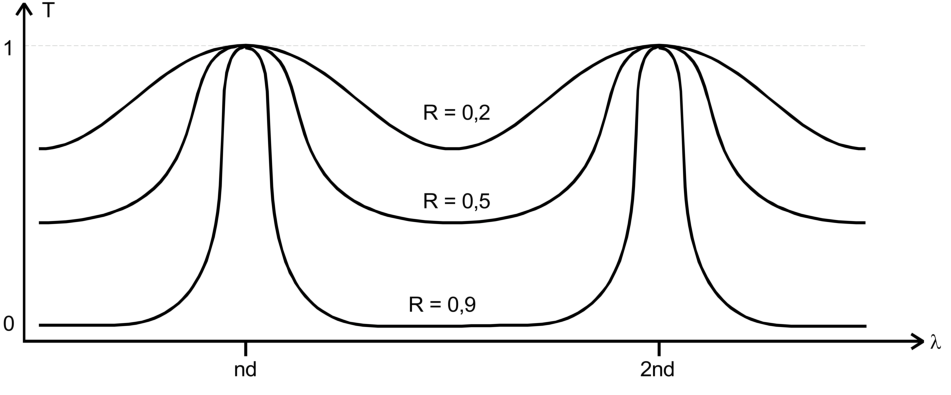
\includegraphics[width=\textwidth]{Pics/Airy.pdf}
  \caption{Verlauf der Transmissionskurve eines Interferenzfilter für verschiedene
  Reflexionskoeffizienten. \cite{anleitung}}
  \label{fig:Airy}
\end{figure}

\subsubsection{Glan-Thompson-Prisma}

Als Polarisatoren werden in diesem Experiment Glan-Thompson-Prisma verwendet.
Es handelt sich dabei um doppelbrechende Kristalle, bei denen die Diagonalelemente
der dielektrischen Suszeptibilität unterschiedlich sind. Analog zu Kapitel
\ref{subsec:Doppelbrechung} können zur Bestimmung der Phasengschwindigkeit
drei Komponentegleichungen formuliert werden:
\begin{align}
  k^2E\ua{x} &= \frac{\omega^2}{c^2}(1+\chi\ua{xx})E\ua{x}
  \label{eqn:GTPx}\\
  k^2E\ua{y} &= \frac{\omega^2}{c^2}(1+\chi\ua{yy})E\ua{y}
  \label{eqn:GTPy}\\
  0 &= \frac{\omega^2}{c^2}(1+\chi\ua{zz})E\ua{z}
  \label{eqn:GTPz}
\end{align}
Aus Formel \eqref{eqn:GTPz} folgt erneut $E\ua{z} = 0$. Für $E\ua{x}\neq 0$ ergibt
sich erneut
\begin{equation}
  v\ua{Ph,1} = \frac{c}{\sqrt{1+\chi\ua{xx}}}.
  \label{eqn:vPhx}
\end{equation}
Unter dieser Annahme lässt sich Gleichung \eqref{eqn:GTPy} wegen $\chi\ua{xx}\neq\chi\ua{yy}$
nur für $E\ua{y}=0$ lösen. Somit handelt es sich hier um eine linear polarisierte
Welle. Analog ergibt sich $E\ua{x}=0$, wenn man zuerst $E\ua{y}\neq 0$ wählt.
Es handelt sich also um eine Aufspaltung in zwei Strahlen, die aufgrund unterschiedlicher
Phasengeschwindigkeiten senkrecht zueinander polarisiert sind.
